\documentclass{article}
\usepackage{oconnor}
\usepackage{ wasysym }

%% UPDATE these variables:
\renewcommand{\hwnum}{1}
\title{CSCI 338, Quiz 03}
\author{Patrick O'Connor}
\collab{n/a}
%%\date{due: 15 January 2021}

\begin{document}

\maketitle

CSCI 338 Computer Science Theory
1 (3 points; due: 10am, May 13)
This is a quiz (not an attendance counting), so you should 
try your best.Note also that this is an open book quiz, 
while all physical resources are allowed, resorting for external human 
help constitutes aplagiarism


% ============================================
% ============================================
\nextprob{Question 1}
\collab{n/a}
% ============================================
Design an NFA for the following with the alphabet {0,1}:


(1.1) {$w|w$ contains a substring 1010}
\paragraph{Answer}
Please see figure \ref{fig:num01}
\begin{figure}
    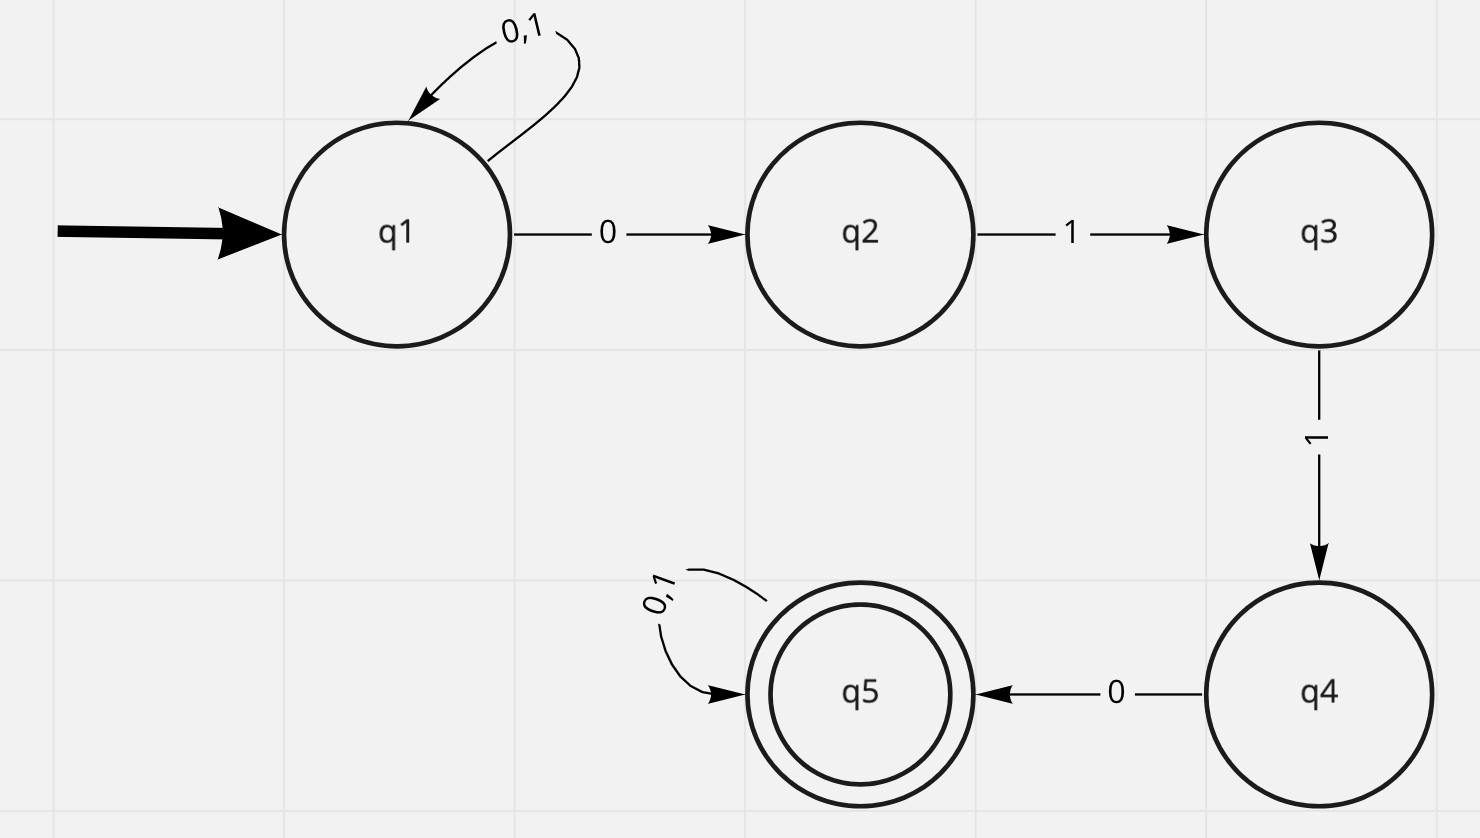
\includegraphics[width=\linewidth]{01-1NFA.png}
    \caption{A NFA for substring 1010}
    \label{fig:num01}
\end{figure}

(1.2) {$w|w$ contains an even number of 0's or exactly two 1's
\paragraph{Answer}
Please see figure \ref{fig:num02}
\begin{figure}
    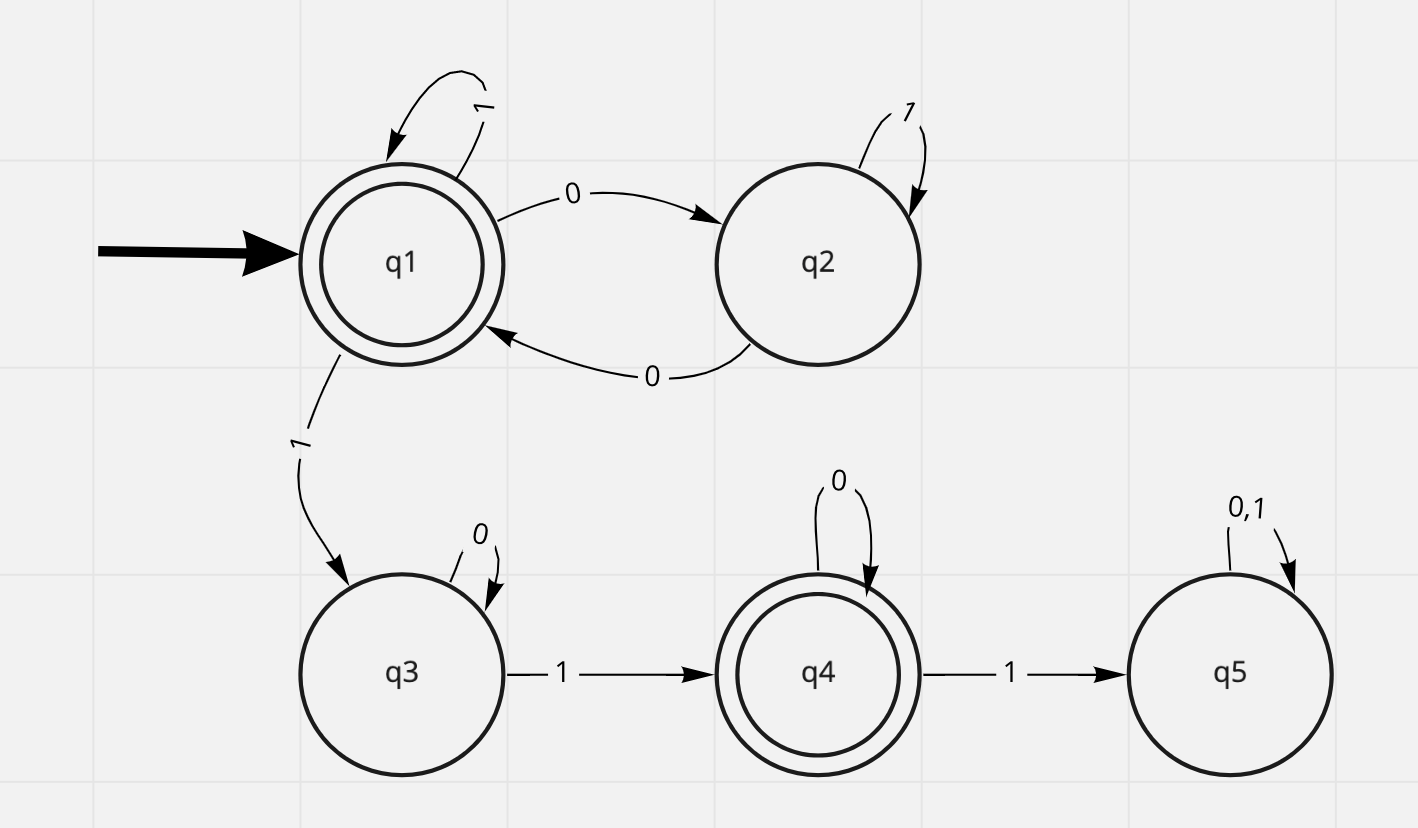
\includegraphics[width=\linewidth]{01-2NFA.png}
    \caption{A NFA that contains an even number of 0's or exactly two 1's}
    \label{fig:num02}
\end{figure}


% ============================================
% ============================================
\nextprob{Question 2}
\collab{n/a}
% ============================================
Using the construction in Thereom 1.39 to convert the following NFA to equivalent DFA.
\paragraph{Proof}
Let $N= (Q, \Sigma, \delta, q_0, F)$ be the NFA recognizing 
some language A.

We can construct a DFA $M= (Q', \Sigma, \delta', q_0', F')$ 
recognizing A. 

\begin{enumerate}
    \item $Q' = P(Q)$ Every state of $M$ is a set of states of $N$. 
    \item For $R \in Q'$ and $a \in \Sigma$, let $\delta'(R,a) = {q \in Q| q 
    \in \delta(r,a)}$ for some $r \in R$ If $R$ is a state of $M$, it is also a set of state $N$.
    Because each state may go to a set of states, we take union of all sets as seen below.
    $\delta'(R,a) = \bigcup\limits_{r \in R} \delta(r,a)$

    \item $(q_0)' = \{q_0\}$ $M$ starts in the state corresponding to the collection containing just 
    the start state of $N$
    \item $F' = \{ R \in Q'|R$ contains an accept state of $N$\}
    The machine $M$ accepts if one of the possible states that $N$ could be in at this point is an accept state.
\end{enumerate}


\end{document}

